\documentclass[10pt]{article}
\usepackage[letterpaper,landscape,margin=0.65in]{geometry}
\usepackage{graphicx}
\usepackage{booktabs}
\usepackage{amsmath}
\usepackage[T1]{fontenc}
\usepackage{hyperref}
\hypersetup{pdftitle={FROB C5 quotient endomorphism controls},
  pdfsubject={EXP-FROB-91ee9c; quotient C5 controls; historical Sage review open}}
\setlength{\parindent}{0pt}
\setlength{\parskip}{0.45em}
\title{FROB C5 quotient endomorphism controls}
\author{Validation audit, 22 October 2026}
\date{}
\begin{document}
\maketitle
\vspace{-2em}

\textbf{Scope.} Lean proves C5 factor-kernel, trace, fifth-power and fixed-line
controls for the actual $q$-power endomorphisms of the three frozen polynomial
quotient algebras. These are ring-level quotient theorems; irreducibility of
the quotient moduli is not assumed or established in Lean.

\begin{center}
\begin{tabular}{lll}
\toprule
Base field & Frozen quotient modulus & Checked endomorphism controls \\
\midrule
$\mathbf F_{11}$ & $z^5+2z^4+1$ & four factor kernels, trace dim $4$, fixed dim $1$ \\
$\mathbf F_{13}$ & $z^5+8z^4+1$ & quartic factor kernel, trace dim $4$, fixed dim $1$ \\
$\mathbf F_{19}$ & $z^5+3z^4+1$ & two factor kernels, trace dim $4$, fixed dim $1$ \\
\bottomrule
\end{tabular}
\end{center}

\textbf{Proof path.} Prior Lean certificates prove all $75$ frozen q-power
matrix entries and the full linear-map equality in each power basis. An
algebra equivalence from endomorphisms to reindexed matrices transports
the exact matrix trace rank $1$ and $M^5=I$ facts. The abstract polynomial
factor identities then apply to the actual q-power maps. Rank-nullity gives
trace-kernel dimension $4$ and fixed-kernel dimension $1$; a fixed vector
in the trace kernel is zero because $5$ is nonzero in each base field.
The aggregate target theorem checks all three cells and their factor-kernel
directness/equality, fifth-power, dimension and disjointness statements.

\textbf{Machine verification.} Source commit \texttt{20982d9a84d8} uses
pinned Lean 4.35.0-rc1. The exact-source verifier passed an 8,976-job full
build and 3,099-job target build, found no forbidden constructs, and audited
686 theorem declarations with standard axioms only. The requested theorem's
axiom audit passed. The JSON receipt records \texttt{machine\_verified};
independent semantic review remains pending.

\textbf{Boundary.} The frozen Sage driver computes the same categories of
matrix and kernel flags, and a separate source-bound Python replay checks
the archived C5 cells. The driver's \texttt{T\_equals\_hM} flag compares
two constructions of the same matrix polynomial and is only a consistency
check. Historical Sage-to-Lean refinement and original execution-source
custody have not been established. Modulus irreducibility in Lean, C8, the
complete experiment gate and performance claims remain open. No scientific
trial or timing run was repeated.

\newpage
\begin{center}
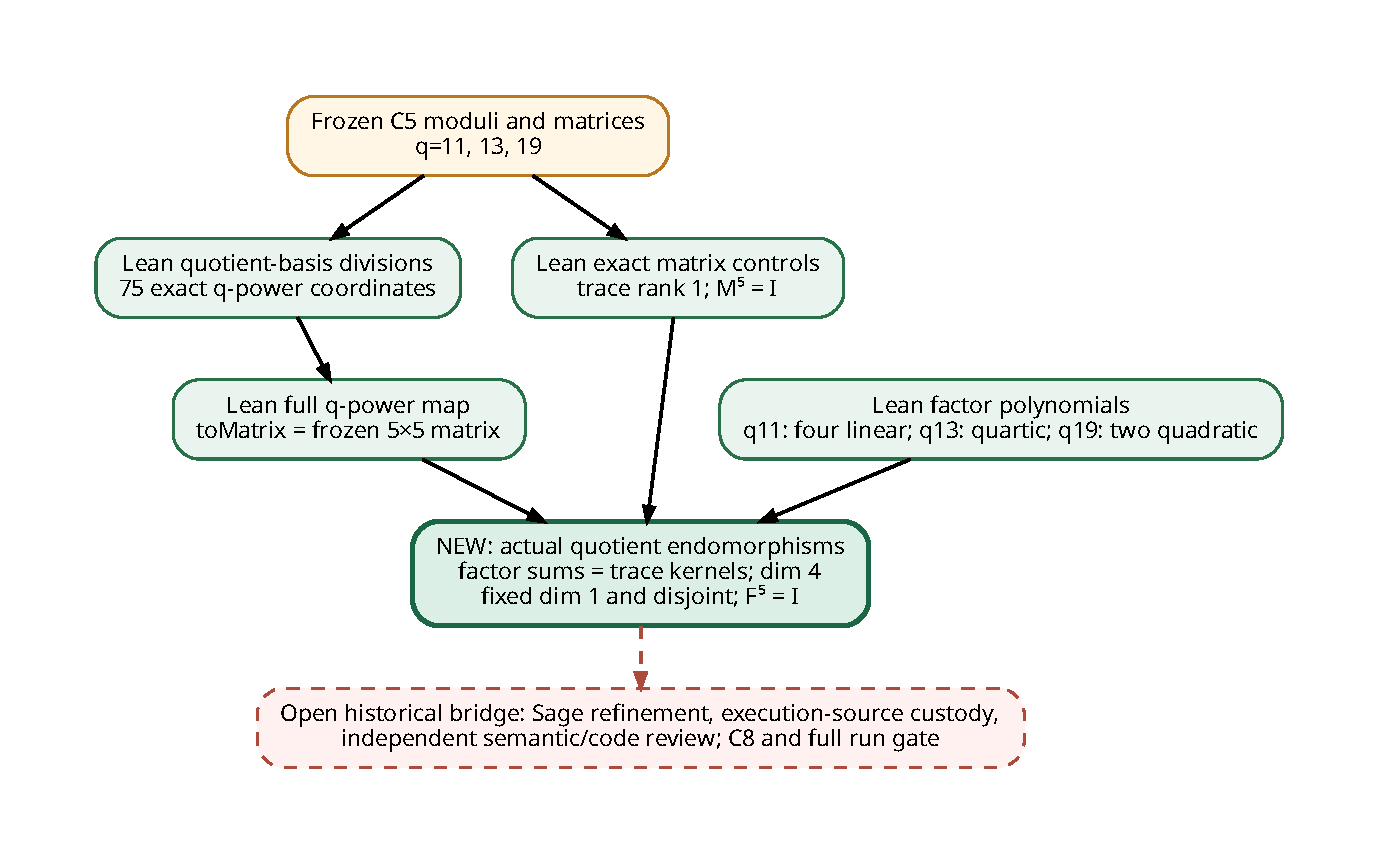
\includegraphics[width=\textwidth,height=0.82\textheight,keepaspectratio]{proof-figure.pdf}
\end{center}
\end{document}
